\documentclass[a4paper,12pt]{article}
\usepackage[utf8]{inputenc}
\usepackage[spanish]{babel}
\usepackage{amsthm}
\usepackage{amsmath}
\usepackage{amsfonts}
\usepackage{pgf,tikz}
\usepackage{graphicx}
\usepackage{float}
\usepackage{cite}
\usepackage{enumerate}
\usepackage{courier}
\usepackage{listings}
\usepackage{color}
\usepackage{physics}
\usepackage{todonotes}

\definecolor{codegreen}{rgb}{0,0.6,0}
\definecolor{codegray}{rgb}{0.5,0.5,0.5}
\definecolor{codepurple}{rgb}{0.58,0,0.82}
\definecolor{backcolour}{rgb}{0.95,0.95,0.92}

\lstdefinestyle{mystyle}{
	backgroundcolor=\color{backcolour},   
	commentstyle=\color{codegreen},
	keywordstyle=\color{magenta},
	numberstyle=\tiny\color{codegray},
	stringstyle=\color{codepurple},
	basicstyle=\footnotesize\ttfamily,
	breakatwhitespace=false,         
	breaklines=true,                 
	captionpos=b,                    
	keepspaces=true,                 
	numbers=left,                    
	numbersep=5pt,                  
	showspaces=false,                
	showstringspaces=false,
	showtabs=false,                  
	tabsize=2
}

\lstset{style=mystyle}
\usepackage{hyperref}
%\graphicspath{ {-} }
\usepackage[toc,page]{appendix}
\newtheorem{theorem}{Teorema}
%opening
\title{Hypothesis testing in biostatistics}

\author{Rubén Hurtado, Bartolomé Ortiz, Cristina Seva }

\begin{document}

\maketitle
\setlength\parindent{0pt}
\begin{abstract}
El presente expone un recorrido por los principales conceptos y fundamentos del contraste de hipótesis. En él proporcionamos un enfoque estadístico de este área centrado en test paramétricos (para una o dos poblaciones normales) y test no paramétricos (recogiendo en particular bondad de ajuste, independencia y localización) . 
\end{abstract}


\section{Base teórica del contraste de hipótesis}
\subsection{Introducción}
El contraste de hipótesis es un área de la inferencia estadística que se ocupa de conocer determinados aspectos de la distribución que tiene nuestro experimento.

Más concretamente, \textit{"la finalidad de un contraste de hipótesis es decidir si una determinada hipótesis, afirmación, o conjetura, sobre la distribución poblacional estudiada, es confirmada o invalidada estadísticamente a partir de las observaciones contenidas en la muestra"}, \cite{velez1993principios}.

En general, en el marco de los test de hipótesis, llamamos \textbf{hipótesis nula} o $\textbf{H}_0$ a la hipótesis que se asume sobre nuestra distribución y la cual se pretende contrastar.
Frente a ella, se propone la \textbf{hipótesis alternativa} o $\textbf{H}_1$, que agrupa aquellas distribuciones que no poseen $H_0$ como cualidad.

Asimismo, también destacamos otra división usual:
\begin{itemize}
	\item \textbf{Hipótesis simples}: son aquéllas que especifican totalmente la distribución poblacional (constituidas por una única función de distribución)
	\item \textbf{Hipótesis compuestas}: Hipótesis  que comprenden varias distribuciones poblacionales 
\end{itemize}

\subsection{Planteamiento general de los contrastes de hipótesis}
Sea $H_0$ la hipótesis nula y $H_1$ la hipótesis alternativa. El problema del contraste de hipótesis consiste en aceptar o rechazar $H_0$.

\subsubsection{Tipos}
Habitualmente, para tomar esta decisión podemos seguir un proceso que puede ser o no aleatorio: 
\begin{itemize}
    \item si se lleva a cabo dividiendo el espacio muestral $\Omega$ en dos regiones distintas: 
	\begin{itemize}
		\item región crítica (rechazo)
		\item región de aceptación 
	\end{itemize} 
	hablamos de test no aleatorio.
	\item Si queremos tener un test aleatorizado: escogeremos una función $\phi$ medible que vaya del espacio de muestra a $[0,1]$ (función crítica del test), de manera que esta función exprese la probabilidad de rechazar la hipótesis nula cuando se observa la muestra $(x_1,...,x_n)$.
	Tendremos pues probabilidad $\phi$ de rechazar $H_0$ y $1-\phi$ de no hacerlo. 
\end{itemize}

\subsubsection{Errores}

    A la hora de realizar un test de hipótesis, hay dos tipos de errores que pueden cometerse.
    El primero, llamado \textbf{error de tipo I}, consiste en rechazar la hipótesis nula $H_0$ cuando ésta es verdadera.
    Por el contrario el otro error, llamado \textbf{error de tipo II}, consiste en no rechazar la hipótesis nula cuando ésta es falsa.

    Los test se caracterizan por la probabilidad de cometer estos errores.
    Por un lado, a la probabilidad de cometer un error de tipo I se la conoce como \textbf{nivel de significación del test}, y suele denotarse con la letra griega $\alpha$.
    Por otro, a la probabilidad de no cometer un error tipo II, esto es, de rechazar $H_0$ cuando esta es falsa, se la conoce como \textbf{potencia del test}.
    La probabilidad de cometer un error de tipo II suele denotarse por $\beta$, de forma que la potencia de un test es $1 - \beta$.

%    En un principio, nos gustaría hacer el nivel de significancia los más pequeño posible a la vez que maximizamos la potencia del test; de forma que minimizásemos la probabilidad cometer cualquier error.
%    Sin embargo, un nivel de significancia muy pequeño implica que aceptamos la hipótesis nula de forma más frecuente, mientras que una potencia elevada implica lo contrario.
%    Por tanto, no podemos alcanzar el objetivo deseado: un menor nivel de significación implicará una menor potencia y viceversa.
%    En consecuencia, será necesario encontrar un compromiso.


\subsubsection{Criterios de elección del test}
    A la hora de plantear o diseñar un test de hipótesis buscamos la disminución de todos los tipos de error; es habitual que esto sea difícil de alcanzar, puesto que disminuir la probabilidad de cometer un erro de tipo I influye positivamente en la probabilidad de cometer error de tipo II. Ante esta amplitud de posibilidades, existe un criterio tradicional para para diseñar los test:
\begin{enumerate}
	\item Fijar un nivel de significación $\alpha$.
	\item Excluir todos los test que no impongan que la probabilidad de rechazar $H_0$ cuando es cierta no supere el valor de $\alpha$ . 
	\item  Entre los test no excluidos por la condición anterior, elegir aquél que maximice la potencia del test.
\end{enumerate}

    Este criterio hace que habitualmente $\alpha$ sea mucho menor que $\beta$. 
    En consecuencia, mientras que el rechazo de $H_0$ implicará que $H_1$ es cierta, el no rechazo de $H_0$ no es suficiente para afirmar esta se verifique.
    


\subsubsection{Valor $p$}
    Cuando realizamos un test a un nivel de significación dado, obtenemos una respuesta binaria: aceptamos o rechazamos.
    Sin embargo, podría interesarnos saber cómo de seguro es el rechazo o aceptación obtenidos, es decir, cuantificar la significación estadística del test (ya que $\alpha$ sólo nos da una cota).
    
    Para esto se utiliza el concepto de \textbf{valor $p$}, que no es más que el nivel de significación en el límite entre la aceptación y el rechazo.
    De esta forma si, por ejemplo, en un test $p= 0.02$, sabemos que rechazaremos $H_0$ siempre que el nivel de significación sea mayor a $0.02$.


\section{Test paramétricos para una población normal}

     Dentro de los distintos tipos de test estadísticos, los \textbf{tests paramétricos} son aquellos en los que se asume cierta distribución para la muestra y se contrasta el valor de sus parámetros.
     Concretamente, nosotros nos centraremos en el caso en el que la muestra sigue una distribución normal.
     
\subsection{Introducción}
En el marco de los problemas paramétricos, el criterio descrito para la selección de test puede formularse como:


\textit{
    Si la distribución teórica depende de un parámetro $\theta \in \Theta$ acerca del cual hay que contrastar la hipótesis nula $H_0: \theta \in \Theta_0$ frente a la alternativa $H_1: \theta \in \Theta_1$ se denomina función de potencia, $\beta(\theta)$, de un test a la probabilidad de rechazar $H_0$ cuando el valor del parámetro es $\theta$. Es decir, si se trata de un test no aleatorizado de región crítica C entonces: $$\beta(\theta)=P_\theta(C)$$
mientras que en general, para un test de función crítica $\phi$, es $$\beta(\theta)=E_\theta[\phi(X_1,...,X_n)].$$
Un test tiene nivel de significación $\alpha$ si es:  $$\beta(\theta)\leq\alpha \text{ para cada } \theta \in \Theta_0;$$
y se denomina tamaño del test al número: 
\begin{equation}
    \mathrm{sup}_{\theta\in\Theta_0}\beta(\theta)
    .
\end{equation}
Es deseable que tamaño y nivel de significación coincidan, verificándose: 
$$\mathrm{sup}_{\theta\in\Theta_0}\beta(\theta)=\alpha$$ }


Una vez tenemos los conceptos básicos en cuanto al contraste de hipótesis, vamos a ofrecer un pequeño recorrido por los test paramétricos que están relacionados con las distribuciones normales.


 \subsection{Contraste $t$ de Student}
 El test $t$ de Student o Test-T es cualquier prueba en la que el estadístico utilizado tiene una distribución $t$ de Student si la hipótesis nula es cierta.
 
 Este test se suele utilizar cuando la población estudiada sigue una distribución normal pero el tamaño muestral es demasiado pequeño como para que el estadístico en el que está basada la inferencia esté normalmente distribuido, utilizándose una estimación de la desviación típica en lugar del valor real. 
 
 En la bioestadística podemos tener casos en los cuales nuestro tamaño de muestra sea pequeño. Esto por ejemplo puede darse en medicina cuando tratamos a grupo reducido de pacientes.

 \subsubsection{Contraste $t$ de una muestra para la media de una distribución normal con varianza desconocida (media alternativa $<$ media hipótesis nula)}
 
 En este caso enfrentamos la hipótesis de que nuestros datos tengan una determinada media, frente a la posibilidad  de que la media sea menor:
 \begin{itemize}
 	\item $H_0:\mu = \mu_0$
 	\item $H_1: \mu < \mu_0$
 \end{itemize}
considerando además que la varianza nos es desconocida.

A este tipo de test  en el que el valor del parámetro en la hipótesis alternativa puede que ser mayor o menor, pero no ambos, se le llama \textbf{contraste unilateral}.
 
 En este caso el estadístico para nuestro test es: 
 $$t=\frac{\bar{x}-\mu_0}{s/\sqrt{n}},$$
 donde $\bar{x}$ es la media muestral, $s$ es la raíz cuadrada de la cuasivarianza muestral y $n$ el tamaño de la muestra.

 Puede probarse que, bajo la hipótesis nula, el estadístico anterior está distribuido según una $t$ de Student con $n - 1$ grados de libertad.
 A partir de esta información y dado un nivel de significación $\alpha$, podemos encontrar la región crítica para este estadístico.
 Dado que $\alpha$ es la probabilidad de rechazar $H_0$ cuando esta es cierta, la probabilidad, bajo $H_0$ de obtener un valor del estadístico $t$ en la región crítica debe ser $\alpha$.

 Como hemos asumido que la media de la distribución debe ser menor o igual que $\mu_0$, esto se traduce en el siguiente criterio:
 \begin{itemize}
 	\item si $t<t_{n-1,\alpha}$, rechazamos $H_0$
 	\item si $t<t_{n-1,\alpha}$, aceptamos $H_0$
 \end{itemize}
 en el que $t_{m, p}$ es el cuantil de orden $p$ de la distribución $t$ de Student con $m$ grados de libertad. Para obtener estos valores deberemos usar una tabla de la distribución $t$ de Student o un ordenador.

 Añadimos también que el $p$-valor podría calcularse vía:
 $$p_{valor}=P[t_{n-1}\leq t].$$

 
 \subsubsection{Contraste $t$ de una muestra para la media de una distribución normal con varianza desconocida. \\ Media alternativa $>$ media nula.}
 En este caso enfrentamos la hipótesis que completa el estado anterior, es decir, queremos saber si nuestros datos tienen una determinada media, frente a la posibilidad  de que la media sea mayor: 
 \begin{itemize}
 	\item $H_0:\mu=\mu_0$
 	\item $H_1: \mu >\mu_0$
 \end{itemize}
 donde de nuevo consideramos que la varianza nos es desconocida.
 
 En este caso el estadístico para nuestro test es el mismo que en el anterior:
 $$t=\frac{\bar{x}-\mu_0}{s/\sqrt{n}}$$
 y lo que cambia son las regiones crítica y de aceptación:
 \begin{itemize}
 	\item si $t>t_{n-1,1-\alpha}$, rechazamos $H_0$
 	\item si $t\leq t_{n-1,1-\alpha}$, aceptamos $H_0$
 \end{itemize}

 Nuevamente, el $p$-valor podría calcularse vía:
 $$p_{valor}=P[t_{n-1}> t]$$
 
 \subsubsection*{Caso práctico en bioestadística}
 (De \cite{rosner2015fundamentals}) 
Supongamos que estamos examinando el nivel de colesterol de $n=10$ niños cuyos padres murieron de una enfermedad cardiaca. Mediante las pruebas encontramos que la media de nuestra muestra es de 200 mg/dL con una desviación típica de 50 mg/dL. Suponemos que es un parámetro que se distribuye como una normal, pero nuestro grupo es demasiado pequeño, por lo que usamos un test $t$ de Student para comparar si la media de colesterol es significativamente mayor aquí que en la población general, la cual posee 175 mg/dL de media.
Planteamos por tanto el problema:
\begin{itemize}
	\item $H_0:\mu=175$
	\item $H_1: \mu > \mu_0$
\end{itemize}
Con nivel de significación $\alpha=0.05$
$$t=\frac{200-175}{50/\sqrt{10}}=\frac{25}{15.81}=1.58$$
ahora comprobamos:
$$t<t_{n-1,1-\alpha}=t_{9,0.95}=1.8333$$
Por lo que aceptamos la hipótesis nula.

\subsubsection{Contraste $t$ de una muestra para la media de una distribución normal con varianza desconocida. Alternativa bilateral}
Es habitual no poder encajar los test de hipótesis en test unilaterales sobre la distribución. 
En estos casos recurrimos a \textbf{tests bilaterales} en los que se busca comprobar la igualdad o desigualdad de un parámetro.

En este caso enfrentamos la hipótesis de que nuestros datos tengan una determinada media, frente a la posibilidad de que esta tome cualquier otro valor:
\begin{itemize}
	\item $H_0:\mu=\mu_0$
	\item $H_1: \mu\neq \mu_0$
\end{itemize}
donde otra vez la varianza nos es desconocida.

El estadístico es el mismo que en los casos anteriores:
$$t=\frac{\bar{x}-\mu_0}{s/\sqrt{n}}.$$
Un vez obtenido, elegimos un nivel de significación $\alpha$ y finalmente:

Lo que cambia es la región de rechazo, que repartimos (arbitrariamente) por igual entre las colas de la distribución
\begin{itemize}
	\item Si $|t|>t_{n-1,1-\alpha/2}$, rechazamos $H_0$
	\item Si $|t|\leq t_{n-1,1-\alpha/2}$, aceptamos $H_0$.
\end{itemize}

La obtención del p-valor para este caso es más complicada:
$$p_{valor} = \begin{cases} 2P[t_{n-1}\leq t], & \mbox{si } t\leq 0 \\ 2(1-P[t_{n-1}\leq t]), & \mbox{si } t>0 \end{cases}$$

\subsection{Contraste bilateral $\chi^2$ para la varianza de una distribución normal}

Terminamos la sección de test para una sola población aportando un caso en el que nos interesa la varianza de la población que suponemos normal.

En este caso enfrentamos la hipótesis de que nuestros datos tengan una determinada varianza, frente a la posibilidad  de que la varianza no sea la esperada: 
\begin{itemize}
	\item $H_0:\sigma^2=\sigma^2_0$
	\item $H_1: \sigma^2\neq\sigma^2_0$
\end{itemize}
donde la media $\mu$ de la distribución es desconocida.

Ahora el estadístico es:
    $$X^2=\frac{(n-1)s^2}{\sigma_0^2}$$
que viene aproximado por una distribución $\chi^2$ con $n - 1$ grados de libertad.
Elegido un nivel de significación $\alpha$, el criterio de aceptación es:
\begin{itemize}
	\item Si $X^2<\chi^2_{n-1,\alpha/2}$ ó $X^2>\chi^2_{n-1,1-\alpha/2}$, rechazamos $H_0$
	\item Si $\chi^2_{n-1,\alpha/2}\leq X^2\leq\chi^2_{n-1,1-\alpha/2}$, aceptamos $H_0$
        ,
\end{itemize}
    donde $\chi^2_{m, p}$ representa el cuantil de orden $p$ de la distribución $\chi^2$ con $m$ grados de libertad.

    Para encontrar estos valores podemos usar una tabla de la distribución $\chi^2$ o un ordenador.

\subsubsection*{Caso práctico en bioestadística}
(De \cite{rosner2015fundamentals}) 
    Para la medida de la presión diastólica y sistólica se usan los llamados sonidos de Korotkov. 
    Estos son unos sonidos característicos que se oyen cuando la presión del brazalete de medida alcanza una presión igual a la sistólica (sonido de Korotkov de primera fase) y a la diastólica (sonido de Korotkov de quinta fase).

    Hay dos formas de analizar estos sonidos: pueden ser escuchados directamente por el personal médico o representados gráficamente para su análisis visual.
    Se espera que el segundo método, al permitir un estudio más cuantitativo, presente una menor variabilidad al ser usado por diferentes observadores.
    Sin embargo, por ser este método más novedoso, el personal médico tiene menos experiencia y podría darse que su uso llevase a una mayor variabilidad entre observadores.

    Para discernir qué es lo que ocurre realmente, recurrimos a un contraste de hipótesis. 
    Asumimos que la diferencia entre las medidas de los observadores sigue una distribución normal con ambos métodos, y que la varianza de esta normal supone una medida adecuada de la variabilidad entre observadores.
    En el caso del método tradicional se sabe que la varianza de la diferencia entre medidas es $\sigma_0^2=35 \; (\textrm{mmHg})^2$.
    Con respecto al nuevo método contamos con los datos de las medidas realizadas por dos observadores a 10 personas diferentes, que muestran una varianza muestral $s^2 = 8.178 \; (\textrm{mmHg})^2$.

    Con estos datos, y dado que no sabemos si el nuevo método supone un aumento o disminución de la variabilidad, recurrimos a un test bilateral con las siguientes hipótesis nula y alternativa:
    \begin{equation}
        H_0 : \sigma^2 = \sigma_0^2, \;
        H_1 : \sigma^2 \neq \sigma_0^2
    \end{equation}
    donde $\sigma^2$ es la varianza de la diferencia de medidas en el nuevo método.

    Siguiendo el proceso descrito anteriormente, empezamos calculando el estadístico $X^2$:
    \begin{equation}
        X^2
        =
        \frac{(n-1)S^2}{\sigma_0^2}
        =
        \frac{(10 - 1) 8.178}{35}
        =
        2.103
        .
    \end{equation}

    Si usamos un nivel de significación $\alpha = 0.05$, los valores críticos son $\chi^2_{9, 0.025} = 2.70$ y $\chi^2_{9,0.975} = 19.02$. 
    Dado que $X^2$ cae fuera de la región de aceptación, rechazamos $H_0$.
    Es decir, la variabilidad de los dos métodos es diferente.
    


\section{Tests paramétricos para dos poblaciones normales}

    Además de los contrastes anteriores, para una sola población, podemos realizar contrastes con varias poblaciones.
    En este caso no se asumen conocidos los valores de ninguno de los parámetros, sino que son comparados entre las dos poblaciones.

\subsection{Contraste $t$ para dos poblaciones independientes con varianzas iguales}
\label{sec:t_2samplessamevar}

    Sean dos poblaciones distribuidas mediante dos distribuciones normales con varianzas desconocidas pero iguales y con tamaños $n_1$ y $n_2$ respectivamente.
    Bajo estas condiciones suponemos que queremos comprobar si sus medias son iguales, esto es hacer el siguiente contraste de hipótesis:
\begin{itemize}
	\item $H_0:\mu_1=\mu_2$
	\item $H_1:\mu_1\neq \mu_2$
\end{itemize}
para un nivel de significación $\alpha$.

En este caso el estadístico que tendremos que utilizar es: 
\begin{equation}
    t
    =
    \frac{\bar{x}_1-\bar{x}_2}{s\sqrt{\frac{1}{n_1}+\frac{1}{n_2}}}
\end{equation}
donde definimos $s$ como:
\begin{equation}
    s=\sqrt{\frac{(n_1-1)s_1^2+(n_2-1)s_2^2}{n_1+n_2-2}}
\end{equation}
y en el que $\bar{x}_i$ y $n_i$ son la media muestral y el tamaño de la muestra de la población $i$.

Este estadístico vendrá distribuido según una $t$ de Student con $n_1 + n_2 - 2$ grados de libertad.

Un vez obtenido el valor del estadístico, concluimos el contraste según:
\begin{itemize}
	\item Si $t > t_{n_1+n_2-2,1-\alpha/2}$ ó $t < -t_{n_1+n_2-2,1-\alpha/2}$, rechazamos $H_0$
	\item Si $-t_{n_1+n_2-2,1-\alpha/2}\leq t\leq t_{n_1+n_2-2,1-\alpha/2}$, aceptamos $H_0$
\end{itemize}
%Para el cálculo final seguimos los mismos procedimientos que en el apartado para una población.\todo{??}

\subsection{Contraste $F$ para dos poblaciones independientes }
\label{sec:F_2samples}
Acabamos la sección de test paramétricos presentando un test para el contraste de hipótesis relacionadas con la igualdad de la varianza de dos poblaciones normales.

    Sean dos poblaciones distribuidas mediante dos distribuciones normales con medias $\mu_1$ y $\mu_2$ y  tamaños $n_1$ y $n_2$ respectivamente.
    Bajo estas condiciones queremos contrastar la hipótesis:
    \begin{itemize}
	\item $H_0:\sigma^2_1=\sigma^2_2$
	\item $H_1:\sigma^2_1\neq \sigma^2_2$
    \end{itemize}
    para un nivel de significación $\alpha$.

    En este caso el estadístico que utilizaremos es: 
    $$F=\frac{s_1^2}{s_2^2}$$
    Bajo la hipótesis nula, este estadístico sigue una distribución $F$ de Snedecor y con parámetros $(n_1 - 1)$ y $(n_2 - 1)$.

    Un vez obtenido el valor del estadístico, concluimos mediante:
    \begin{itemize}
	\item Si $F>F_{n_1-1,n_2-1.1-\alpha/2}$ o $F<F_{n_1-1,n_2-1.1-\alpha/2}$, rechazamos $H_0$
	\item Si $F_{n_1-1,n_2-1.1-\alpha/2}\leq F \leq F_{n_1-1,n_2-1.1-\alpha/2}$, aceptamos $H_0$
    \end{itemize}

    Para el cálculo final seguimos los mismos procedimientos que en el apartado para una población, utilizando la tabla de la distribución F de Snedecor.

    Este test resulta útil en los casos en los que se quiere comprobar la igualdad de varianzas para aplicar a posteriori el test $t$  de la media presentado en la sección \ref{sec:t_2samplessamevar}.


%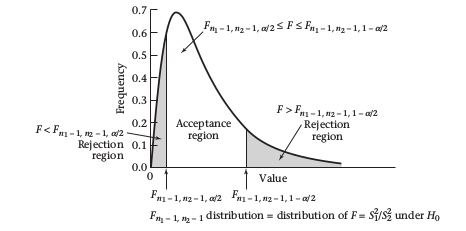
\includegraphics{ejemplo_grafica.png}

\subsubsection*{Caso practico en bioestadística}
 (De \cite{rosner2015fundamentals}) 
Supongamos que queremos comparar el nivel de colesterol en sangre de dos colectivos, que suponemos distribuidos por dos distribuciones normales $N(\mu_1, \sigma_1^2)$ y $N(\mu_2, \sigma_2^2)$.
    El primer colectiva presenta una muestra y varianza muestral de $\bar{x}_1 = 207.3 (\textrm{mg/dL})$, $s_1 = 35.6 (\textrm{mg/dL})$, mientras que el segundo $\bar{x}_2 = 193.4 (\textrm{mg/dL})$, $s_2 = 17.3 (\textrm{mg/dL})$.
    Sus tamaños son, respectivamente, $n_1 = 100$ y $n_2 = 74$.
    Para ello, queremos aplicar el test $t$ introducido en la sección~\ref{sec:t_2samplessamevar} para ver si sus medias son iguales.
    Sin embargo, no podemos hacer esto si no sabemos previamente que $\sigma_1^2 = \sigma_2^2$.
    Así, hemos de empezar realizando el test $F$ descrito en la sección \ref{sec:F_2samples}.

    Las hipótesis en este caso son:
    \begin{equation}
	H_0:\sigma^2_1=\sigma^2_2; \quad H_1:\sigma^2_1\neq \sigma^2_2
    \end{equation}
    Y el estadístico a comprobar:
    $$F
    =
    \frac{s_1^2}{s_2^2}
    = 
    \frac{207.3^2}{193.4^2}
    =
    4.23
    $$

    Tomando un nivel de confianza $\alpha = 0.05$, pasamos a calcular los valores críticos del estimador:
    \begin{equation}
        F_{99,\, 73,\, 0.975} = 1.54908
        ; \quad
        F_{99,\, 73,\, 0.025} = 0.65476
    \end{equation}

    Dado que el estimador queda fuera de la región de aceptación, rechazaríamos la hipótesis nula y no podríamos utilizar el test $t$ para comparar las medias.
    
   

\section{Contrastes globales sobre la distribución poblacional (test no paramétricos)}

\subsection{Introducción}
En muchas ocasiones es necesario emitir un juicio estadístico sobre la distribución poblacional en su conjunto, por ejemplo:
\begin{itemize}
\item Ante una muestra aleatoria de una población, ¿puede admitirse que la distribución poblacional coincide con una dada? Problema de la bondad del ajuste
\item Teniendo varias muestras aleatorias simples (m.a.s.), ¿puede admitirse que provengan de la misma distribución teórica? Problema de homogeneidad
\item Se observan dos o más características de los elementos de una población, son independientes? Problema de la independencia.
\end{itemize}

Se distinguen dos tipos de planteamientos, a saber:
\begin{enumerate}
    \item Descomponer el recorrido de la distribución teórica en un número finito de subconjuntos y clasificar las observaciones muestrales según el conjunto al que pertenezcan. Después, comparar las frecuencias observadas de cada subconjunto con las que corresponderían a la distribución teórica. Esto da lugar a los test $\chi^2$, los cuales reducen un problema no paramétrico a uno que sí lo es.
\item Usar la distribución muestral $F^*_n(x)$ para compararla con la distribución teórica o para compararlas entre sí si es un problema de independencia. Midiendo la distancia entre ambas puede saberse si es o no significativa siempre que se tenga un patrón
\end{enumerate}

\subsection{Contrastes $\chi^2$ de bondad del ajuste}
\subsubsection*{Hipótesis simple} 
Se dispone de una m.a.s. de tamaño $n$ de una población con distribución desconocida $F$. Se quiere contrastar si puede aceptarse la hipótesis $H_0 : F = F_0$ donde $F_0$ es una distribución especificada (no paramétrica). La hipótesis alternativa $H_1$ se trata entonces de todas las distribuciones distintas a $F_0$.

El recorrido de la distribución poblacional se divide en $k$ conjuntos disjuntos $A_1,...,A_k$. Sea $p^0_i$ la probabilidad de cada $A_i$ bajo $F_0$ y $p_i$ la probabilidad desconocida que la distribución teórica asigna a cada $A_i$:

La variable aleatoria que cuenta el número de observaciones de la muestra en cada subconjunto tiene distribución multinomial con parámetros $n$ (tamaño de muestra) y $\textbf{p}= (p_1,...,p_k)$:
$$P\{n_1,..., n_k\}= \frac{n!}{n_1!\cdots n_k!} p^{n_1}_1\cdots p^{n_k}_k,$$
donde $n_i$ es el número de observaciones en cada subconjunto $A_i$.

Se ha logrado pues pasar a un test paramétrico de $H_0 :   \textbf{p} = \textbf{p}^0$ frente a la hipótesis de que el parámetro sea otro.

Por tanto, esto se puede resolver por un test de razón de verosimilitudes, aunque la tradición clásica hace que se utilice habitualmente un test $\chi^2$, dado que este es anterior en el tiempo. Este además aporta los mismos resultados que el de razón de verosimilitudes.
%el estadístico a usar normalmente sea otro que da los mismos resultados \todo{cuál??}. Esto se debe a que el test de razón de verosimilitudes es posterior a los test $\chi^2$.

El estadístico a usar en este caso es:
\begin{equation}
    D = \sum_{i=1}^k \frac{(n_i - n p^0_i)^2}{n p^0_i}
    ,
\end{equation}
que bajo la hipótesis nula viene aproximada (para $n$ grande) por una distribución $\chi^2$ con $k - 1$ grados de libertad.
Con esto, podemos construir la región crítica y realizar el test.


\subsubsection*{Hipótesis compuesta} 
La situación habitual es que la hipótesis a contrastar sea compuesta; más concretamente se especifica una familia de distribuciones con forma funcional dada pero dependiente de algunos parámetros no especificados.

Se podría pensar en hacer los dos test por separado, i.e., realizar la estimación puntual de los parámetros para contrastar después el ajuste a la distribución poblacional que indiquen los propios datos como la más adecuada, pero para ello se necesitarían dos m.a.s. independientes.

Alternativa: Contrastar una hipótesis nula de la forma $F \in \{F_\theta| \theta \in \Theta \subset R^q\}$, donde $\theta$ representa una elección de los $q$ parámetros de la distribución y $\Theta$ el conjunto de parámetros considerados en la hipótesis nula.
En este caso primero se obtiene por máxima verosimilitud la estimación del $\theta$ adecuado en $\Theta$. Una vez hecho esto se procede de igual manera que con la hipótesis simple, terminando por comparar paramétricamente una distribución multinomial.
Nótese que en este caso el estimador tendrá que ser comparado con una distribución de $k - 1 - q$ grados de libertad.

\subsection{Contraste $\chi^2$ de homogeneidad}
%¿Tenemos $m$ muestras de tamaños $n_1, n_2,...,n_m$ o bien una única muestra de tamaño $n_1+n_2+\cdots + n_m$?
Dadas $m$ muestras de tamaños $n_1, n_2,...,n_m$ nos podemos preguntar: ¿vienen éstas de la misma distribución poblacional?


Al ser un test $\chi ^2$ el procedimiento es el mismo que en la sección anterior. Empezamos por dividir en subconjuntos y clasificar las observaciones de cada muestra. La hipótesis nula aquí es que la probabilidad de cada subconjunto $A_j$ en la muestra $i$, $p_{ij}$, no dependa de la muestra elegida; esto es:
\begin{equation}
    p_{ij} = p_i, \quad \forall j
    .
\end{equation}

El estimador a considerar aquí es:
\begin{equation}
    D
    =
    \sum_{i=1}^m \sum_{j=1}^k
            \frac{(n_{ij} - n_i n_{\cdot j}/n)^2}{n_i n_{\cdot j}/n}
    ,        
\end{equation}
en el que $n_{ij}$ es la frecuencia del subconjunto $A_j$ en la muestra $i$, $n_i$ el tamaño de la muestra $i$ y $n_{\cdot j}$ la frecuencia del subconjunto $A_j$ al considerar todas las muestras.
Este estimador vendrá distribuido según una distribución $\chi^2_{(m-1)(k-1)}$ bajo la hipótesis nula.




\subsection{Contraste $\chi^2$ de independencia}
    Se tienen $n$ elementos de una población en los que se observan 2 características, $X$ e $Y$ obteniéndose una m.a.s. bidimensional $(X_1,Y_1),...,(X_n,Y_n)$, ¿son estas características independientes? La forma de proceder vuelve a ser análoga a las anteriores, lo que nos demuestra la versatilidad de los test $\chi^2$.

    En este caso dividiremos los datos en subconjuntos $k\cdot r$ en función de el valor de $X$ y de $Y$ ($k$ subconjuntos en $X$ y $r$ subconjuntos en $Y$).
    Llamaremos $n_{ij}$ al número de elementos de la muestra  que están simultáneamente en el subconjunto $A_i$ de $X$ y $B_j$ de $Y$, $n_{\cdot j}$ a los que están en $B_j$ (independientemente del valor de $X$) y $n_{i \cdot}$ a los que están en $A_i$ independientemente de $Y$.

    La hipótesis nula será que para todo $i$, $j$:
    \begin{equation}
        p_{ij} = p_{i \cdot} p_{\cdot j}
    \end{equation}
    con $p$ la probabilidad en la distribución poblacional y los subíndices siguiendo la misma notación que la $n$.

    Con esta notación, el estimador a usar en este caso es:
    \begin{equation}
        D
        =
        \sum_{i=1}^k \sum_{j=1}^r
                \frac{(n_{ij} - n_{i\cdot} n_{\cdot j}/n)^2}
                {n_{i \cdot} n_{\cdot j}/n}
        ,        
    \end{equation}
    que bajo la hipótesis nula sigue una distribución $\chi^2_{(k-1)(r-1)}$.



\subsection{Contraste de Kolmogorov-Smirnov }
Pese a su versatilidad, los tests $\chi^2$ tienen algunas desventajas: al discretizar las observaciones muestrales en conjuntos de una cierta partición, en el caso de las distribuciones continuas se ignora el valor exacto de las observaciones, lo que puede dar lugar a errores significativos en caso de que la muestra no sea lo suficientemente grande.

Por tanto, para el caso de bondad del ajuste a una distribución unidimensional de tipo continuo es preferible el uso de un procedimiento alternativo: en lugar de estudiar la diferencia entre los histogramas de frecuencias se compara la función de distribución muestral con la función de distribución teórica.

La función de distribución muestral asociada a una muestra aleatoria $x_1, x_2,..,x_n$ es 
$$F^*_n(x) = \frac{(\textrm{nº de $x_i$}) \leq x}{n} = \left\{ \begin{array}{lcc}
             0 &   si  & x \leq x_{(1)} \\
             \\ i/n &  si & x_{(i)} < x < x_{(i+1)} \\
             \\ 1 &  si  & x \geq x_{(n)}
             \end{array}
   \right. $$
donde $x_{(1)},...,x_{(n)}$ son los elementos de la m.a. ordenada.

Si estamos frente a una muestra aleatoria simple de una población descrita por la variable aleatoria $X$ con función de distribución $F$, por el \textbf{Teorema de Glivenko-Cantelli} se tiene que hay probabilidad 1 de obtener una sucesión muestral con la cual $F^*_n(x)$ converja a $F(x)$ uniformemente en $x$, i.e.,
$$\sup |F^*_n(x) - F(x)| \xrightarrow{c.s.} 0$$
% esto se tiene que poder escribir mejor

Teniendo en cuenta que $F$ es desconocida y que se pretende contrastar la hipótesis nula $H_0 : F_0 = F$ usaremos como estadístico
$$\Delta_n = \sup |F^*_n(x) - F(x)|  $$
y por tanto tendremos como región crítica $\{\Delta_n > k\}$. Aunque esto de poco sirve si no se conoce la distribución de $\Delta_n$ bajo la hipótesis nula, necesaria para determinar el nivel crítico $k$ a partir del cual sus valores son significativos de la existencia de una desviación de $F$ respecto a $F_0$.

\begin{theorem}
(Lema) Si $F = F_0$ y $F_0$ es continua, la distribución de $\Delta_n$ no depende de $F_0$
\end{theorem}
Con la demostración se da una expresión integral de la distribución buscada que no proporciona un resultado explícito pero que permite tabular la distribución de $\Delta_n$ para valores pequeños de $n$.

Para valores grandes de $n$ se puede usar la distribución $K$ de Kolmogorov:
$$P\{\sqrt{n}\Delta_n \leq z \} \longrightarrow \sum^{\infty}_{k=-\infty} (-1)^{k} e^{-2k^2 z^2}  $$
que fue tabulada por Smirnov.

Puesto que los resultados sobre la distribución de $\Delta_n$ provienen de suponer que la distribución poblacional es continua, es obvio que sólo se podrá utilizar este test en este tipo de distribuciones.

Como pega, comentar que para hipótesis compuestas es necesario tener dos muestras independientes, cosa que no pasaba con los test $\chi^2$.



\subsection{Contraste de homogeneidad de Kolmogorov-Smirnov}

Se dispone de dos muestras aleatorias simples independientes, $X_1,...,X_n $ e $Y_1,...,Y_m$ y se quiere contrastar la hipótesis nula $H_0:F_X = F_Y$.

Si dichas distribuciones son de tipo continuo, los tests $\chi^2$ tienen los mismos problemas que en la sección anterior y sólo podrían usarse para muestras grandes.

Para muestras pequeñas, se usará la misma técnica de los estadísticos de Kolmogorov-Smirnov. Considerando
\begin{center}
$F^*_n (x)=\frac{1}{n}\sum_{i=1}^n I_{\{X_i \leq x\}}$ y $G^*_n (x)=\frac{1}{m}\sum_{i=1}^m I_{\{Y_i \leq x\}}$
\end{center}
construimos el estadístico de Kolmogorov-Smirnov correspondiente a ambas muestras $$\Delta_{n,m}=\sup|F^*_n(x)-G^*_m (x)|$$
Contrastamos la hipótesis $H_0$ con un test de región crítica $\{ \Delta_{n,m} > k\}$.

La distribución del estadístico $\Delta_{n,m}$ se pueden determinar por métodos combinatorios, aunque también están tabulados para $n$ y $m$ pequeños.

Para $n$ y $m$ grandes, se puede usar los resultados de la distribución asintótica de Kolmogorov:
$$P\left\{ \sqrt{\frac{nm}{n+m}}\Delta_{n,m}\leq z\right\}\longrightarrow \sum^{\infty}_{i=-\infty}(-1)^i e^{-2i^2z^2}$$


\subsection{Contrastes de Independencia}
Para contrastar la independencia entre dos características poblacionales continuas $X$ e $Y$, hay otras opciones como el test $\tau$ de Kendall, el test de rachas o el test de coeficiente de correlación entre rangos de Spearman.

\subsection{Contrastes de Localización}
Dada una distribución unidimensional desconocida de una población, en ocasiones sólo interesa conocer su posición sobre la recta ya que se presupone que las condiciones en que se observa el fenómeno sólo pueden trasladarla, dejando invariante su forma.

Si puede admitirse la normalidad de las distribuciones, la manera de proceder sería aplicando test paramétricos sobre la media de una normal. Sin embargo, cuando no quepa esta posibilidad, lo habitual es el uso de la mediana muestral para contrastar hipótesis sobre las medianas poblacionales.

\subsubsection{Test de los signos}
Se trata de una prueba no paramétrica para comparar el rango medio de dos muestras relacionadas y determinar si existen diferencias entre ellas. Es una alternativa al test $t$ de Student cuando no se puede suponer la normalidad de las muestras.

Se dispone de una muestra aleatoria simple de tamaño $n$ proveniente de una distribución continua pero desconocida $F$ cuya mediana se denotará por $M$. Se quiere contrastar la hipótesis nula $H_0: M=m_0$ frente a una de las alternativas, ya sea $M<m_0$, $M>m_0$ o simplemente $M\neq m_0$.

Por definición, $F(M)=1/2$ por lo que si $H_0$ se cumple, cabe esperar que en torno a la mitad de las observaciones estén por debajo de $m_0$ y la otra mitad esté por encima. Basaremos por tanto el contraste en el estadístico

\begin{center}
$T$ = número de observaciones muestrales mayores que $m_0$.
\end{center}

Notar que $T$ sigue una distribución binomial de parámetros $n$ y $1/2$ bajo la hipótesis nula.

La región crítica va a depender de cuál sea $H_1$, por ejemplo, si $H_1:M>m_0$, cuando $H_0$ no sea cierta, la muestra tenderá a presentar más valores superiores a $m_0$ de los esperados, por lo que la región crítica será de la forma:
$$\{T\geq k \},$$
con $k$ tal que $\frac{1}{2^n}\sum_{j=k}^{n} \binom{n}{j} < \alpha$ para que el contraste tenga nivel de significación $\alpha$. Esto es análogo para el caso $H_1: M< m_0$.

Sin embargo, para algo más general como es el caso de $H_1:M\neq m_0$, el test debe rechazar valores muy altos y muy bajos de $T$, de manera que la región crítica será 
    $$\{T\leq k\}\cup \{T\geq n - k \},$$
con $k$ tal que $\frac{1}{2^n}\sum_{j=1}^{k} \binom{n}{j} + \frac{1}{2^n}\sum_{j=n-k}^{n} \binom{n}{j} \leq \alpha$, siendo $\alpha$ el nivel de significación.

Si el tamaño muestral es lo suficientemente grande, puede emplearse la aproximación normal a la distribución binomial.

\subsubsection{El test de Wilcoxon de los rangos signados}
En el caso de que la distribución pueda considerarse simétrica, además de continua, Wilcoxon propuso un test para la misma hipótesis que el test de los signos, es decir, $H_0:M =m_0$ que saca más provecho de los valores de las observaciones.

Llamemos $D_i=X_i - m_0$ a las diferencias entre las observaciones muestrales y el valor a contrastar para $M$. Podemos ordenar los valores absolutos $|D_i|$ y anotar el rango $r(|D_i|)$ que cada uno ocupa en la ordenación.  Entonces podemos usar como estadístico de contraste la suma de los rangos de las observaciones mayores que $m_0$:
$$T^+ = \sum_{i =1}^{n} r(|D_i|)I_{\{D_i>0\}}.$$

Si se cumple la hipótesis alternativa $H_1:M>m_0$, parece razonable esperar que haya más diferencias positivas que negativas y que las positivas tengan valores absolutos superiores a las negativas. Es decir, habrá que rechazar la hipótesis alternativa si $T^+$ tiene un valor alto, lo que nos lleva a tomar como región crítica $\{T^+ > k_1\}$. El resultado es simétrico para la hipótesis $H_1:M<m_0$.

Para la hipótesis más general $H_1: M \neq m_0$, la región crítica es $\{ T^+<k\}\cup\{T^+ >k'\}.$

Si llamamos $a_n(t)$ al número de asignaciones de signos a los rangos que hace $T^+=t$ se tiene $$P\{T^+ = t\}=\frac{a_n(t)}{2^n}$$ 





\section{Aplicación en Bioinformática:}
\large{Identificación de Genes Responsables de Rasgos Cuantitativo \textit{(QuantitativeTrait Loci, QTLs)}}
\normalsize{}
\subsection{Contexto biológico}
Tras los ejemplos que se han podido observar a lo largo del texto sobre aplicaciones en bioestadística, en especial en el campo de la salud, queremos profundizar en algún aspecto que nos acerque al estudio bioinformático para complementar nuestro trabajo.

En este caso, la temática escogida es el uso que se le pueden dar a los test de hipótesis en la identificación de genes responsables de rasgos cuantitativos. Aunque todo el estudio de este procedimiento se sale un poco del trabajo, queremos aportar una visión global de este problema biológico y el acercamiento estadístico hacia su solución basándonos en \cite{uned2}.

La problemática se centra en el estudio de los rasgos poligenéticos (cuantitativos), es decir, características fenotípicas de los seres vivos que surgen de la interacción de varios genes, además de la posible interacción con el medio ambiente. 
Nuestro objetivo final es detectar donde se encuentran estos genes, que producen cambios en rasgos cuantitativos (los llamados QTLs), pero realmente a priori no sabemos cuáles son. Por tanto, el procedimiento habitual es marcar tramos de la secuencia de ADN (lo que se conoce como marcador genético) y estudiar si entre dos de ellos existen diferencias cuando el rasgo que queremos comprender es diferente. 

Es intuitivo observar que nuestro resultados no pueden quedarse aquí, puesto que los marcadores genéticos pueden contener una gran cantidad de genes distintos. Surge la necesidad de la primera herramienta estadística, que sería una regresión desde el marcador hasta el gen que queremos buscar. Nuestros problemas no acaban ahí, y es que durante la división celular sabemos que se se produce una recombinación genética con lo que la información que nos proporcionan los marcadores puede verse alterada. 
En resumen, para llevar a cabo este estudio analizaremos diferencias entre marcadores genéticos entre dos poblaciones (retrocruzadas\footnote{El retrocruzamiento es un proceso experimental que se lleva a cabo con el fin de obtener individuos homocigóticos (ambos cromosomas idénticos en ambas posiciones)}) que presente dimorfismo en el rasgo que nos interesa, buscando hacer inferencia de las diferencias entre QTLs usando los marcadores.

\subsection{Ejemplos de aplicaciones de test de hipótesis}
La manera más simple de identificar si existe o no un QTL en dos poblaciones, es considerar cada marcador al que tenemos acceso individualmente, dividir los individuos según su genotipo (homocigóticos y heterocigóticos) y, para cada marcador genético, hacer un test de la $t$ de Student de comparación de dos poblaciones (diferenciadas en nuestro caso por el rasgo escogido), puesto que no es descabellado pensar que al tratar con un rasgo cuantitativo en dos poblaciones, éste venga determinado por una distribución normal.

Planteando el problema en un lenguaje más matemático, estamos ante dos expresiones diferentes de un rasgo. En la población 1, el rasgo sigue una distribución $N(\mu_1,\sigma)$ y en la población 2, el rasgo sigue una distribución $N(\mu_2,\sigma)$, siendo la $H_0:$ No existen diferencias significativas entre ambas medias poblacionales (o, más específicamente hablando, no hay una diferencia significativa en los genes del marcador seleccionado\footnote{En realidad la hipótesis nula que vamos buscando es la no existencia de diferencias entre todos los marcadores, pero en esta breve exposición de aplicaciones, no vamos a profundizar a tanto nivel}).
Como podemos ver, es un test de comparación de medias.

Por otra parte, también es habitual realizar test de contraste de hipótesis conocida una región determinada de nuestro marcador. En ese caso se utiliza un estadístico particular LOD (logaritmos de las odd ratio a favor de una relación QTL). Este estadístico, como se expone en \cite{uned2},  tiene una distribución aproximada $\chi^2$
con lo que podremos utilizar los test para esta distribución.
Sin embargo, como apuntábamos, si queremos centrarnos en todo el genoma, debemos modificar estos test y con ello los estadísticos en los que se basan. 

Exponemos así que lo dicho en el trabajo es solo una pincelada de las aplicaciones de los test de hipótesis y también de la teoría estadística en la que yacen. Conforme surgen nuevos problemas en biología y en especial en bioinformática con su actual auge, la estadística también debe evolucionar.


\bibliographystyle{apalike}
\bibliography{bibliography/bibliografia}

\end{document}
